\documentclass[]{article}

\usepackage{amsmath,amsfonts,graphicx}
\usepackage{multirow}
\usepackage{setspace}
\usepackage[FIGBOTCAP,normal,bf,tight]{subfigure}
\usepackage{wrapfig}
\usepackage{setspace}
\usepackage{tabularx}
\usepackage{comment}
\usepackage{float}
\usepackage{booktabs}

\usepackage{bm}


\newcommand{\uo}{\ensuremath{\mbox{UO}_2}}


% path to figures directory
\graphicspath{
{figures/}
}

\begin{document}

\title{Comparison of Contact Formulations:\\
The Sliding Block Problem}

\author{Fuels Modeling \& Simulation Department\\
Idaho National Laboratory\\
Idaho Falls, ID}
\maketitle


\section{Introduction}
\label{introduction}
This document summarizes the development of heavy tests to investigate the improvements made to the contact system with the introduction of the constraint based contact formulation.  Two types of simulation scenarios were analyzed: sliding contact and in-and-out contact.  For each of these scenarios simulations were run for a variety of contact formulations.  Both constraint and Dirac contact formulations were investigated using kinematic and penalty enforcement of frictionless contact.  In MOOSE modules frictionless contact permits tangential sliding between the contact surfaces as well as release of nodes during tension.  Only penalty enforcement was investigated for constraint and Dirac based contact formulations of frictional (coulomb) contact.  Four different coefficients of friction were analyzed: 0.2, 0.4, 0.6 and 0.8.  A preliminary analysis was completed of kinematic enforcement of frictional contact but it is clear that obtaining convergence is random and as such further development is required in this area.  The purpose of these heavy tests were to investigate the active time, total number of nonlinear iterations, penetration and contact pressure results.  Parallelizability of the contact formulations was also investigated.  All results presented indicate that the contact capabilities within MOOSE modules are currently behaving as expected for this sliding bar problem.  Sixteen (16) tests were added to moose/modules/combined/sliding\_block/.  Tests for both frictionless and kinematic enforcement of frictionless contact for all 4 contact formulations investigated are included.  In addition 2 frictional contact tests are included for each contact formulation which use penalty enforcement of contact and coefficients of friction of 0.2 and 0.4 respectively.

\section{Problem Setup}
\label{problem_setup}

The sliding bar problem consists of a small block sliding down the surface of another much larger block in two-dimensions.  The small block was 0.6 mm wide and 0.8 mm long and the large block was 0.6 mm wide and 20 mm long.  Figure~\ref{fig:sliding_block} illustrates the geometry and mesh used for all analyses.  The mesh contained a total of 146 quadrilateral elements.

\begin{figure}[H]
   \centering
   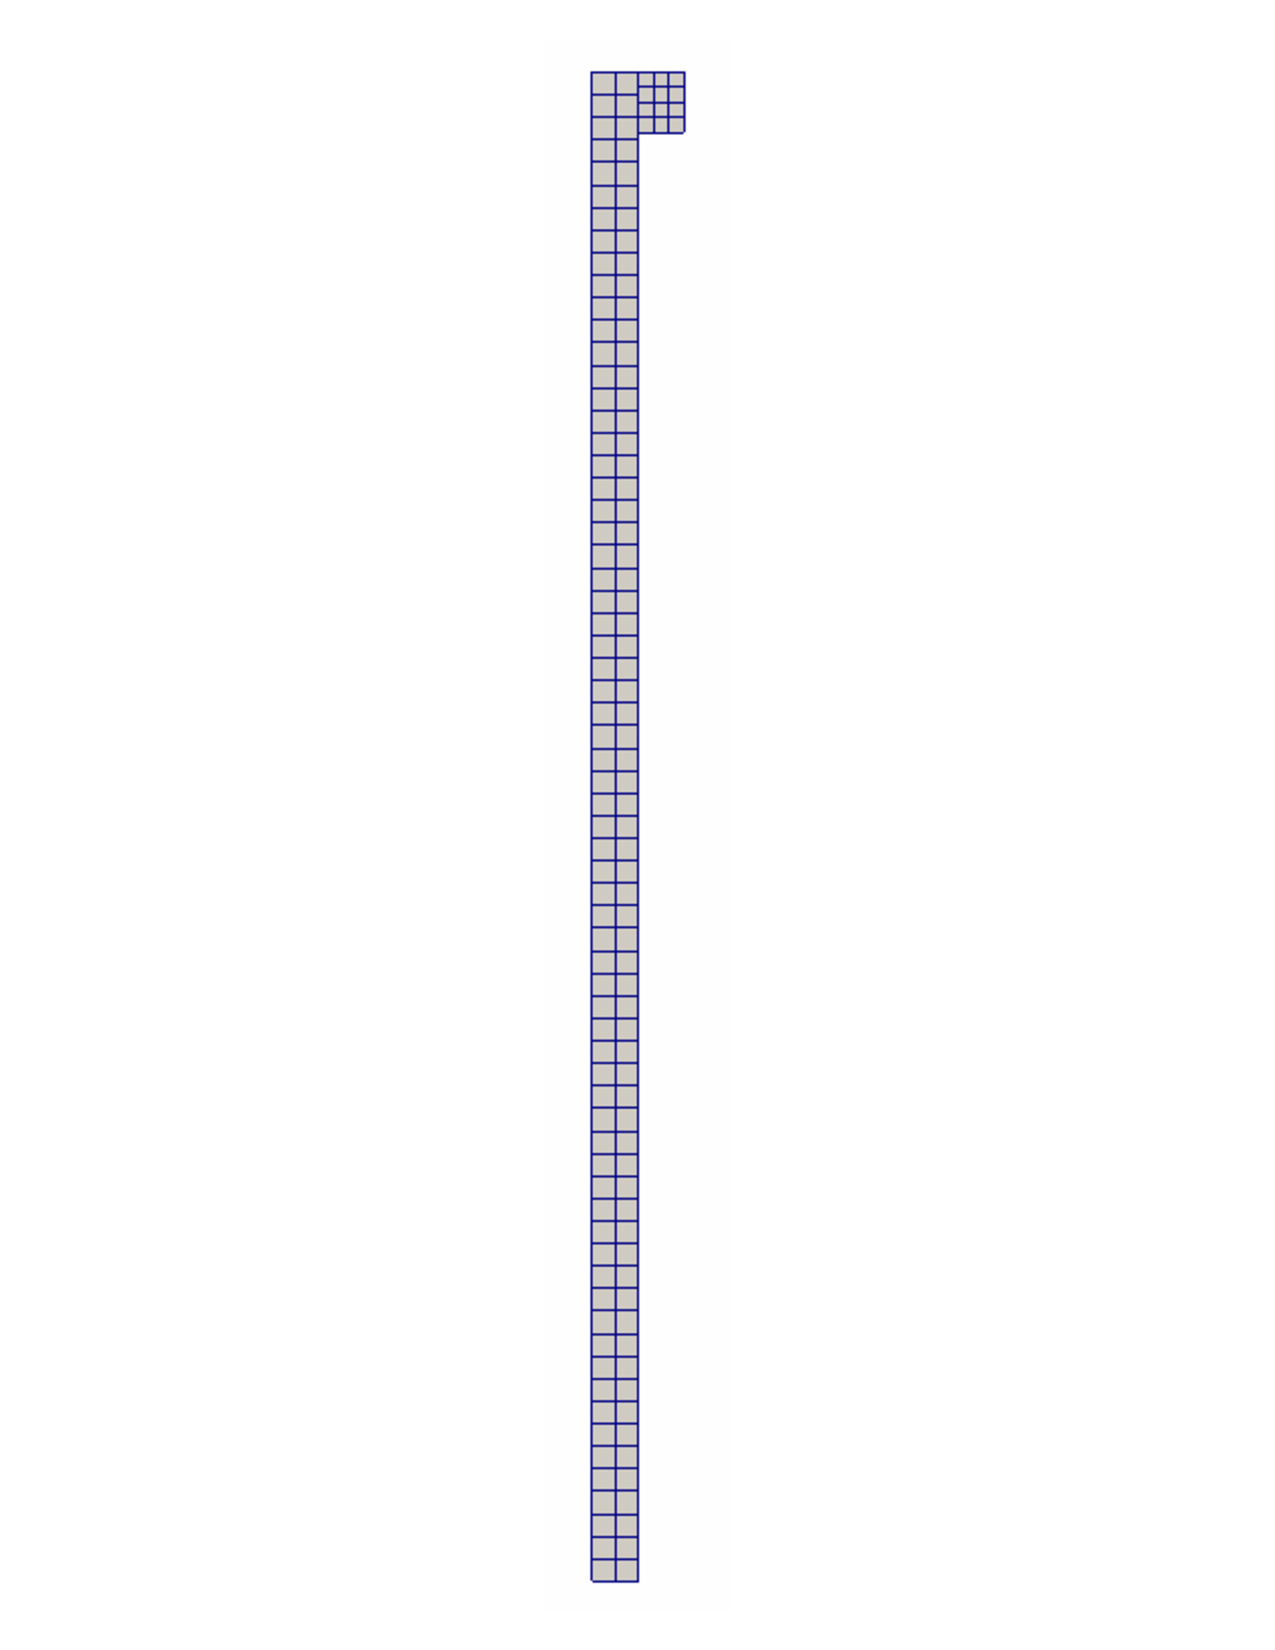
\includegraphics[keepaspectratio, width=5in]{sliding_block}
   \caption{Geometry and mesh used for the sliding block tests.}
   \label{fig:sliding_block}
\end{figure}

\noindent The blocks are modeled as a simple linear isotropic material with a Poisson's ratio of 0.3 and a Young's Modulus of 1e6.  Both blocks are made of the same material.  The blocks initially start apart from one another and then a horizontal and vertical displacement is perscribed to the small block.  Table~\ref{table:displacements} illustrates the functions used to prescribe the displacement of the small block for both sliding and in-and-out contact.  For sliding contact the blocks are moved into contact and never come out of contact for the duration of the simulation, whereas in-and-out contact simulations the small block going into and out of contact as it slides vertical.  This is accomplished by prescribing a sinusoidal function. The duration of the simulation is a total of 15 seconds.  All simulations were run on a Mac Workstation.

\begin{table}[!ht]
\caption{Horizontal and vertical displacements}
\centering
\begin{tabular}{ccc}
\hline
\textbf{Type of} & \textbf{Horizontal} & \textbf{Vertical} \\
\textbf{Contact}  & \textbf{Displacement} & \textbf{Displacement}\\
\hline
sliding & $ -0.02 $ & $ -t + 0.1 $ \\
in-and-out & $ -0.04sin(4t)+0.02 $& $ -t + 0.1$ \\
\hline
\end{tabular}
\label{table:displacements}
\end{table}

\section{Frictionless Contact}
\label{frictionless_contact}

The first set of contact tests that were conducted investigated the frictionless contact.  Both Dirac and constraint based formulations were investigated as well as kinematic and penalty enforcement.  As expected the penetration and contact pressure results were independent of the number of processors used for the simulation.  Simulations were run on 1, 2 and 4 processors to ensure that the solution was invariant among processors used.  There was little to no gain in computational speed and this is due to the fact that the mesh density and number of degrees of freedom in the model were relatively small. Table~\ref{table:fsc_active}  presents the active time results for the frictionless formulation of sliding contact.  From these results it can be seen that for constraint based contact there appears to be very little difference in the run times between penalty and kinematic contact.  A small increase in run time is observed when using Dirac based contact.  Surprisingly even with a small amount of elements the problem sees an decrease in run time on two processors.  Similar trends are observed for in-and-out contact as presented in Table~\ref{table:finc_active}.  The run time increase between constraint and Dirac based formalisms is negligible in the in-and-out case.  The total number of nonlinear iterations were independent of the number of processors used.  466, 431, 482 and 452 nonlinear iterations were required for penalty constraint, kinematic constraint, penalty Dirac and kinematic Dirac enforcement of sliding contact, respectively.  For in-and-out contact the number of nonlinear iterations required were 499, 462, 506 and 467 for penalty constraint, kinematic constraint, penalty Dirac and kinematic Dirac respectively. \\

\begin{table}[!ht]
\caption{Active time in seconds for frictionless sliding contact.}
\centering
\begin{tabular}{cccc}
\hline
\textbf{Type of} & \textbf{One} & \textbf{Two} & \textbf{Four} \\
\textbf{Enforcement}  & \textbf{Processor} & \textbf{Processors} & \textbf{Processors}\\
\hline
Penalty Constraint & 29.135 & 20.957 & 21.784 \\
Kinematic Constraint & 27.894 & 20.969 & 21.242 \\
Penalty Dirac  & 51.898 & 35.584 & 37.966 \\
Kinematic Dirac & 37.592 & 27.109 & 26.634 \\
\hline
\end{tabular}
\label{table:fsc_active}
\end{table}

\begin{table}[!h]
\caption{Active time in seconds for frictionless in-and-out contact.}
\centering
\begin{tabular}{cccc}
\hline
\textbf{Type of} & \textbf{One} & \textbf{Two} & \textbf{Four} \\
\textbf{Enforcement}  & \textbf{Processor} & \textbf{Processors} & \textbf{Processors}\\
\hline
Penalty Constraint & 32.633 & 23.467 & 24.186 \\
Kinematic Constraint & 31.544 & 22.421 & 22.481 \\
Penalty Dirac  & 38.783 & 26.500 & 29.832 \\
Kinematic Dirac & 32.011 & 22.820 & 24.316 \\
\hline
\end{tabular}
\label{table:finc_active}
\end{table}

\noindent The contact pressure and penetration results were determined by obtaining a nodal variable value at Global Node ID 222.  This was to allow comparison of the results among different processes for the same contact parameters and for comparison between the different contact formalisms. Figure~\ref{fig:fric_penetration}  shows the penetration results for the four different enforcement methods analyzed for frictionless sliding contact.  As expected zero penetration is observed for the kinematic cases.  Moreover constraint and Dirac based contact produces identical results for both the penalty and kinematic cases.

\begin{figure}[H]
   \centering
   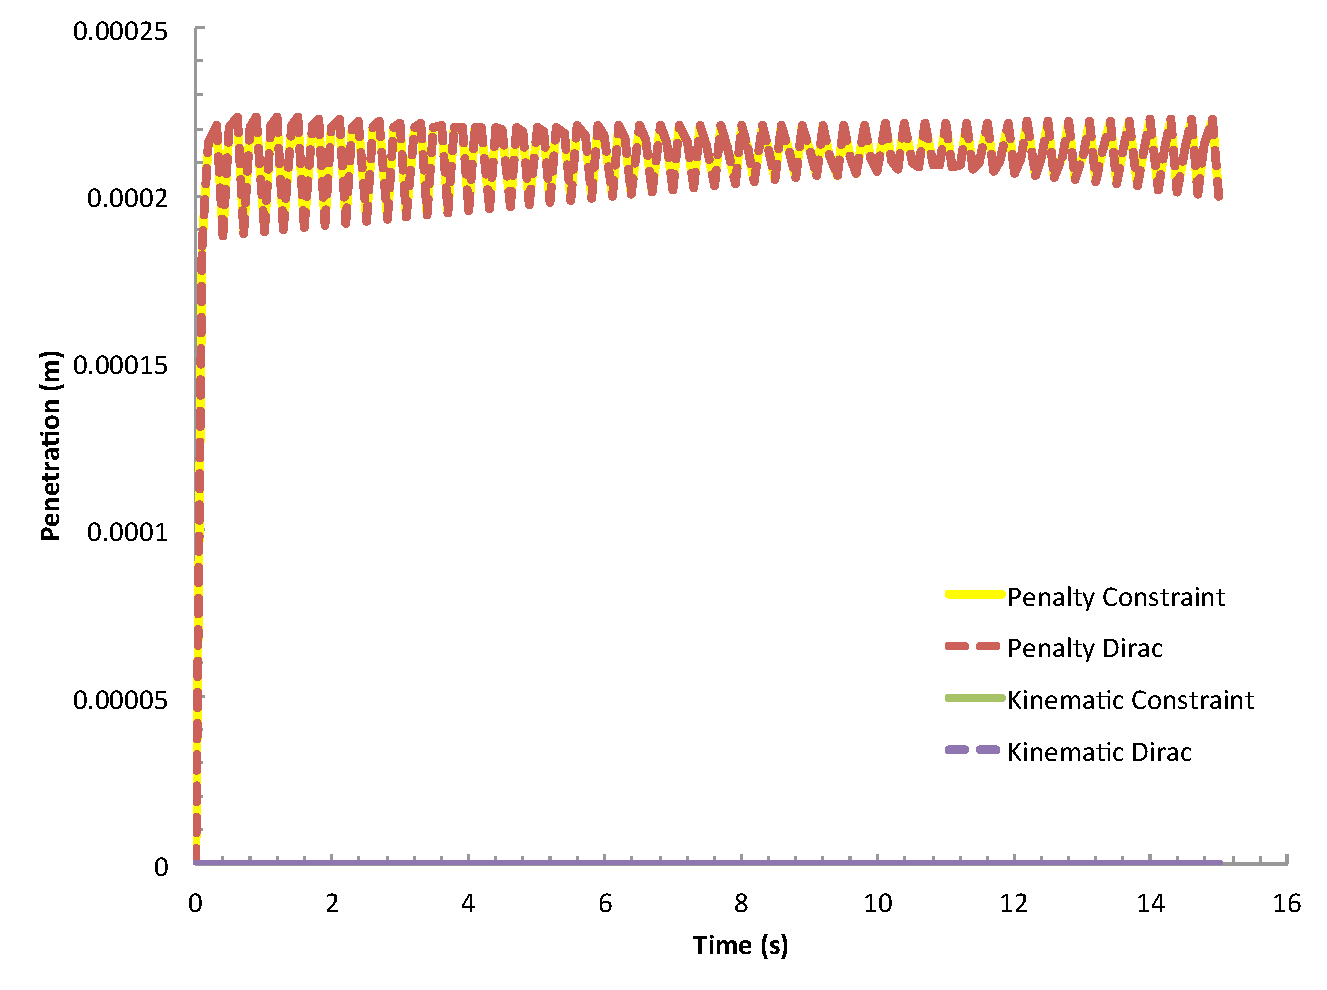
\includegraphics[keepaspectratio, width=4in]{fric_penetration}
   \caption{Penetration results for frictionless sliding contact.}
   \label{fig:fric_penetration}
\end{figure}

\noindent Figure~\ref{fig:fric_inout} shows the penetration results for in-and-out contact for the four different contact formulations analyzed.  The figure zooms on the section near the intersection of the two blocks, denoted as the penetration equals zero line on the graph.  As expected kinematic and penalty enforcement provide identical results when the blocks are not in contact (i.e. negative penetration).  As with sliding contact, when the blocks are in contact the Dirac and contraint formulations provide the same results depending upon whether penalty or kinematic enforcement is used.

\begin{figure}[H]
   \centering
   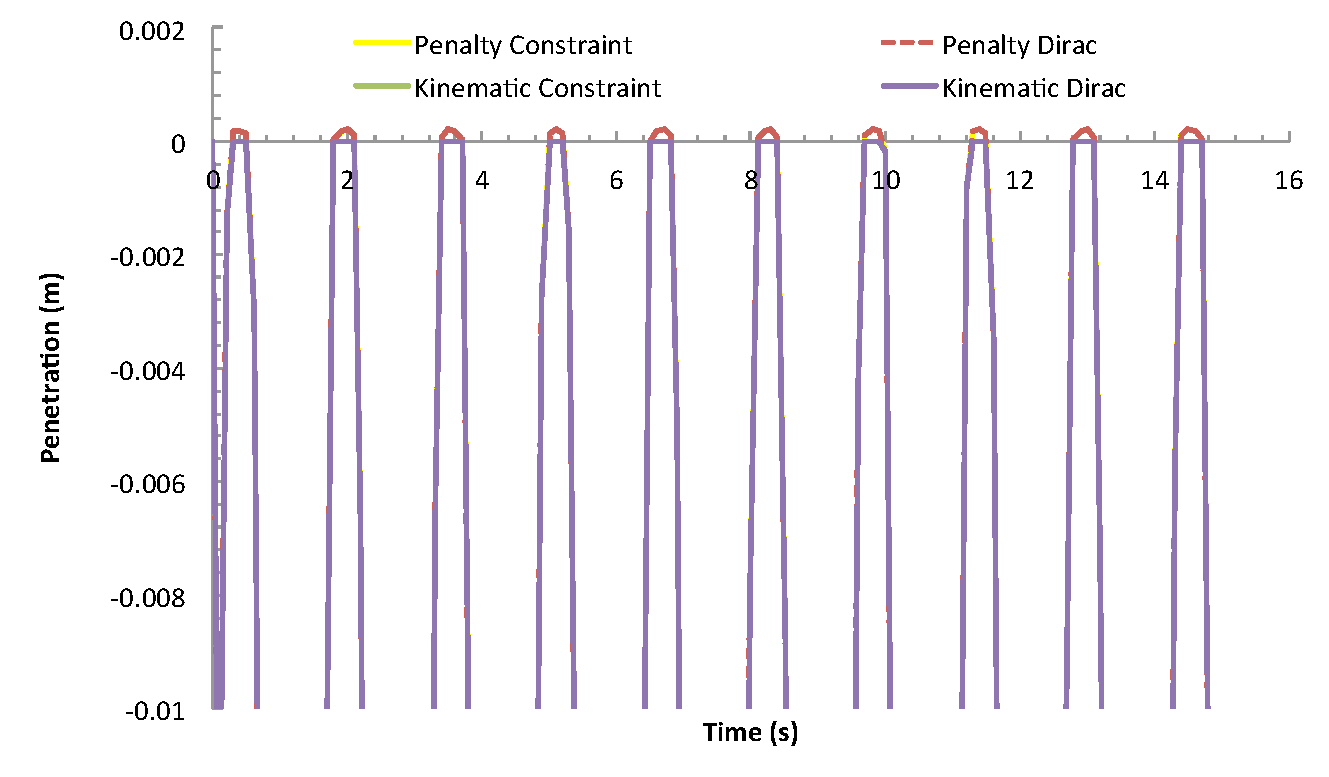
\includegraphics[keepaspectratio, width=4in]{fric_inout}
   \caption{Penetration results for frictionless in-and-out contact.}
   \label{fig:fric_inout}
\end{figure}

\section{Frictional Contact}
\label{frictional_contact}

\noindent The second set of contact tests that were conducted investigated the coulomb friction formulation of contact.  Similarly to the frictionless case both Dirac and constraint based formulations were investigated.  Only penalty enforcement was considered as it was determined that kinematic enforcement of frictional contact is currently not robust and stable.  Further investigation and development is required.  To fully investigate the capabilities of the coulomb friction model four different coefficients of friction were simulated: 0.2, 0.4, 0.6, and 0.8.  This varies the amount of resistance against sliding of the smaller block .  A value closer to 0 approaches frictionless contact whereas a value closer to 1 approaches a glued contact constraint where no tangential sliding or tension release is permitted.  The best way to illustrate the active time comparison for frictional contact is through a graphical figure to compare the results for the differing coefficients of friction.  Figure~\ref{fig:friction_sc_active} presents a graph showing the active time on 1, 2 and 4 processors for all coefficients of friction for constraint based penalty sliding contact.  For a friction coefficient of 0.8 convergence was not able to be obtained on a single processor.  The reason for this is unclear.  Figure~\ref{fig:friction_inc_active} shows the results obtained for constraint based penalty in-and-out contact.  Similar trends are observed when using Dirac contact. It can be seen that the increase in run time as the coefficient of friction increases is more signifcant for in-and-out contact.

\begin{figure}[H]
   \centering
   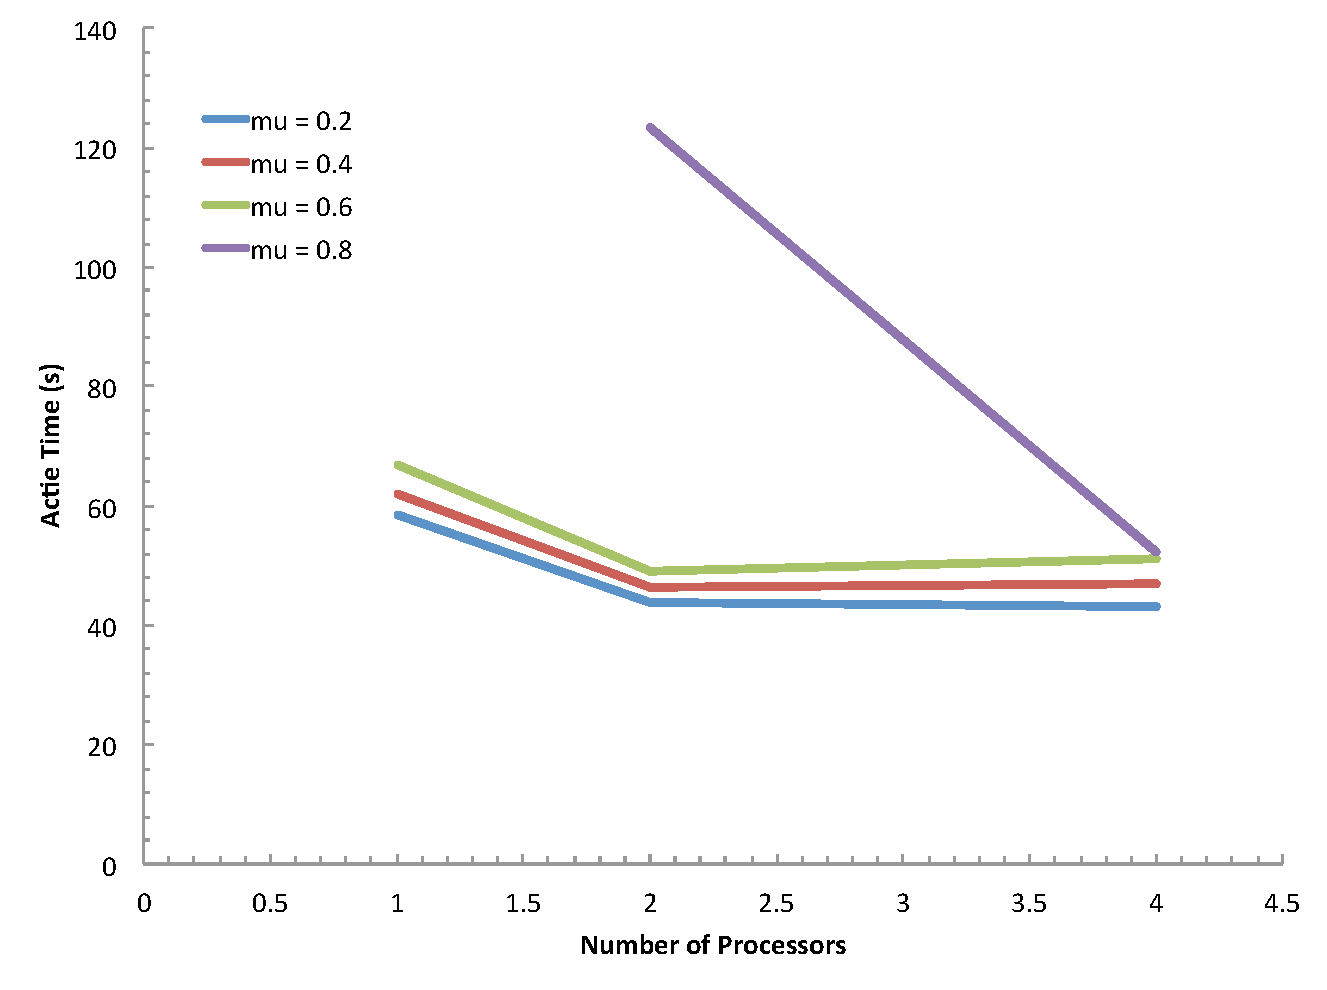
\includegraphics[keepaspectratio, width=4in]{friction_sc_active}
   \caption{Active time results for various coefficiencts of friction using constraint based enforcement of sliding contact.}
   \label{fig:friction_sc_active}
\end{figure}

\begin{figure}[H]
   \centering
   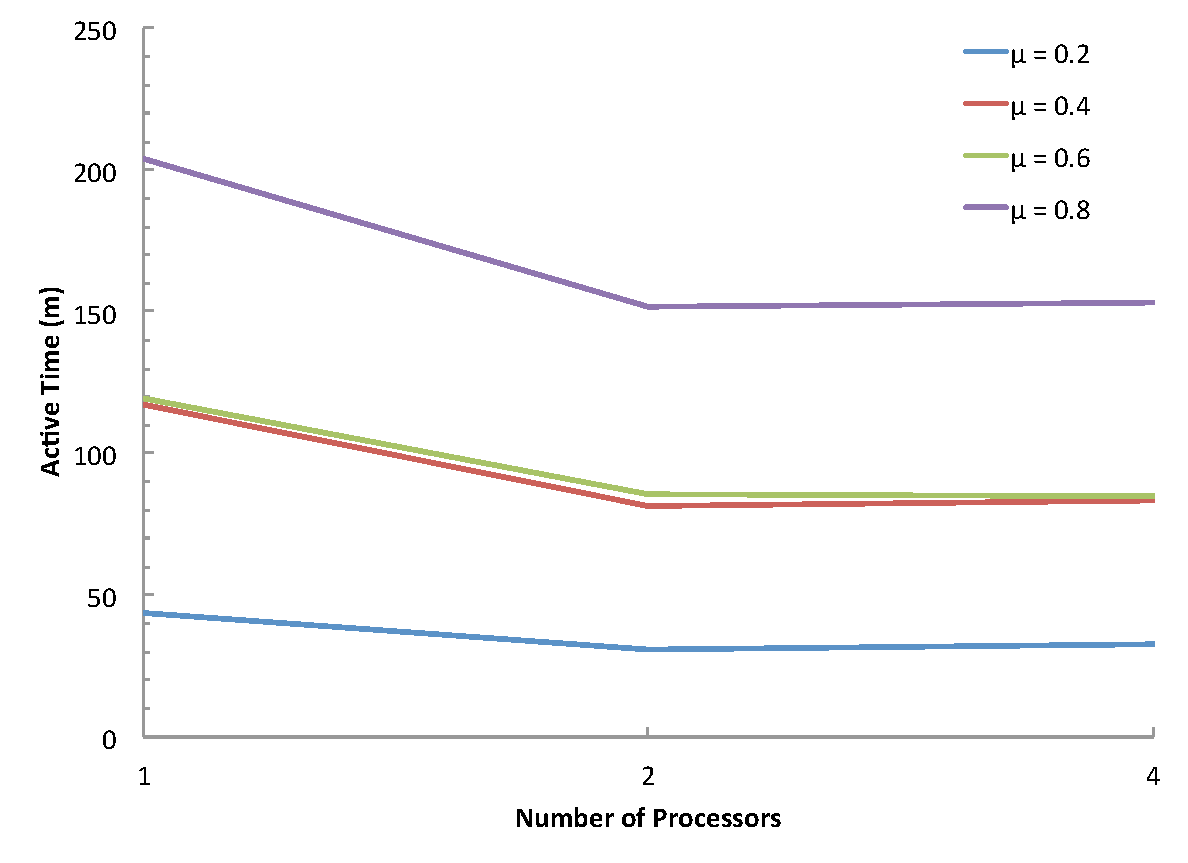
\includegraphics[keepaspectratio, width=4in]{friction_inc_active}
   \caption{Active time results for various coefficiencts of friction using constraint based enforcement of in-and-out contact.}
   \label{fig:friction_inc_active}
\end{figure}

\noindent Tables~\ref{table:sliding_nonlinear} and~\ref{table:inandout_nonlinear} summarize the total nonlinear iterations required for each case.

\begin{table}[H]
\centering
\caption{Total nonlinear iterations for penalty enforcement of frictional sliding contact.}
\begin{tabular}{*9c}
\toprule
Processors &  \multicolumn{4}{c}{Constraint} & \multicolumn{4}{c}{Dirac}\\
\midrule
{}   & $\mu$=0.2   & $\mu$=0.4     & $\mu$=0.6    & $\mu$=0.8 & $\mu$=0.2 & $\mu$=0.4 & $\mu$=0.6 & $\mu$=0.8 \\
1   &  478 & 507   & 548  &          & 454 & 826 & 482 & 934\\
2   &  478 & 507   & 548  & 1074 & 454 & 826 & 482 & 934\\
4   &  478 & 507   & 548  & 613   & 454 & 826 & 482 & 934\\
\bottomrule
\end{tabular}
\label{table:sliding_nonlinear}
\end{table}


\begin{table}[H]
\centering
\caption{Total nonlinear iterations for penalty enforcement of frictional in-and-out contact.}
\begin{tabular}{*9c}
\toprule
Processors &  \multicolumn{4}{c}{Constraint} & \multicolumn{4}{c}{Dirac}\\
\midrule
{}   & $\mu$=0.2   & $\mu$=0.4     & $\mu$=0.6    & $\mu$=0.8 & $\mu$=0.2 & $\mu$=0.4 & $\mu$=0.6 & $\mu$=0.8 \\
1   &  659 & 1052   & 1159  & 1806   & 1145 & 1163 & 644 & 1890\\
2   &  659 & 1052   & 1159  & 1820   & 1145 & 1163 & 644 & 1890\\
4   &  659 & 1052   & 1159  & 1857   & 1145 & 1163 & 644 & 1889\\
\bottomrule
\end{tabular}
\label{table:inandout_nonlinear}
\end{table}

\noindent Due to friction it is expected the small block will deform under shearing forces as it slides down the larger block.  This can be observed in Figure ~\ref{fig:deformation} which illustrates the deformation and the leading edge having a higher contact pressure.  Although the shearing is small in magnitude it can be seen that the surface of the small block that is sliding is lagging slightly behind in vertifcal displacement.

\begin{figure}[H]
   \centering
   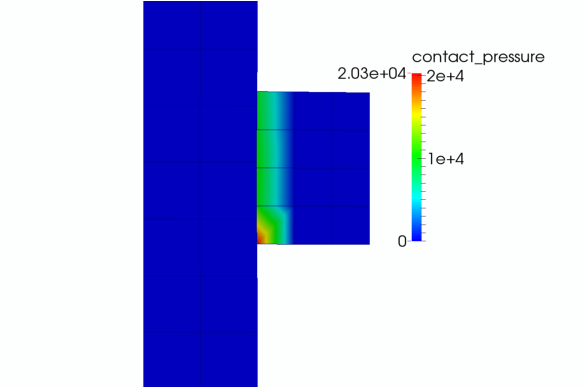
\includegraphics[keepaspectratio, width=4in]{deformation}
   \caption{Deformation of the small block due to friction.}
   \label{fig:deformation}
\end{figure}

\section{Discussion}
\label{discussion}

\noindent The above investigation was completed to investigate the contact behavior observed since the implementation of the new constraint based contact formulation.  A small subset of the tests (16) carried out above were created into heavy tests to be included in MOOSE modules.  The idea is to run these heavy tests nightly to ensure they continue to run as the code develops.  The gold files for these tests were run on one processor and the tests require a minimum of 4 processors to ensure there is no variability in the due to parallelization. \\

\noindent A thorough investigation of kinematic enforcement of frictional contact was not completed due to further development is required.  Initial investigation indicated that constraint based contact solved on a single processor for all friction coefficients investigated for both sliding and in-and-out contact.  However, Dirac based contact had convergence issues (i.e. max iterations hit in a newton solve) for all friction coefficients for in-and-out contact.  Moreoever ever single contact formalism immediately had a segementation fault error at the beginning of the simulation when kinematic enforcement of frictional contact was used on more than one processor.  Heavy tests for kinematic enforcement of frictional contact can be developed and revisited once further developments have been made to make the algorithm more robust and efficient as simulations times are much longer than penalty enforcement when the simulation does converge.

\section{Conclusions}
\label{conclusions}

\noindent In conclusion, the contact algorithms currently present within the MOOSE computational framework are behaving as expected.  Constraint and Dirac contact formulations produce the same results for penalty and kinematic enforcement respectively.  As expected the results are different between penalty and kinematic enforcement.  Moreover when using friction the small block is deformed due to the resistance against sliding as would be expected.  Lastly, further development and investigation of kinematic enforcement of frictional contact is required.

\end{document}
